\section{Potência e Energia}

Considere, por exemplo, uma lâmpada de 100 W que fornece mais luz que uma de 60
W, ou mesmo quando pagamos nossas contas de luz às fornecedoras em que estamos
pagando pela energia elétrica consumida ao longo de certo período. Portanto, os
cálculos de potência e energia são importantes na análise de circuitos. Sendo a
potência a velocidade com que se consome ou se absorde energia, medida em
watts (W).

\begin{equation}
	\label{eq:potencia}
	p \overset{\triangle}{=} \frac{dw}{dt}
\end{equation}

onde \( p \) é a potência em watts (W), \( w \) é a energia em joules (J) e \( t
\) é o tempo em segundos (s). Sendo assim se segue que:

\begin{equation}
	\begin{aligned}
		\label{eq:potencia-instantanea}
		p & = \frac{dw}{dt}                     \\
		  & = \frac{dw}{dq} \cdot \frac{dq}{dt} \\
		  & = vi                                \\
	\end{aligned}
\end{equation}

Chamada \textit{potência instantânea}, a Equação~\ref{eq:potencia-instantanea}
define que a potência é o produto da tensão no elemento pela corrente através
dele. Caso positivo esta potência é absorvida pelo elemento e caso negativa é
fornecida pelo elemento. Isto é chamado de \textit{convenção de sinal passivo} e
pode ser visualizado na Figura~\ref{fig:fig3}:

\begin{figure}[H]
	\centering
	\setlength{\fboxsep}{0pt}
	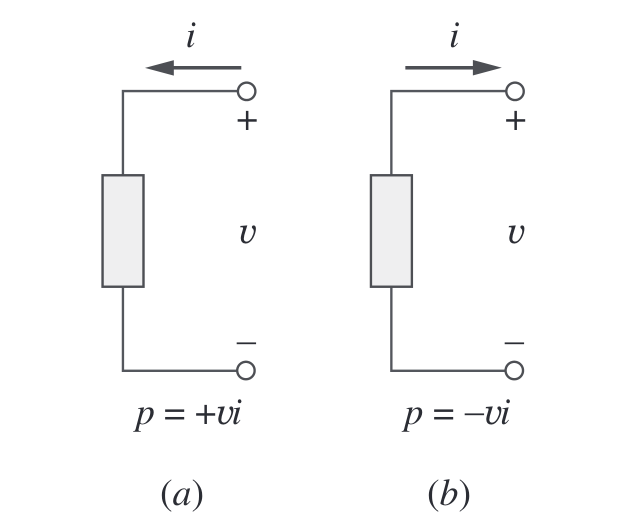
\includegraphics[height=0.15\textwidth]{./fig/fig3.png}
	\caption{Polaridades referenciais para potência usando a convenção do sinal
		passivo: (\( a \)) absorção de potência; (\( b \)) fornecimento de potência.}
	\label{fig:fig3}
\end{figure}

\[
	+\text{Potência absorvida} = –\text{Potência fornecida}
\]

Na realidade, a lei da conservação da energia tem de ser obedecida em
qualquer circuito elétrico. Por essa razão, a soma algébrica da potência em um
circuito, a qualquer instante de tempo, deve ser zero:

\[
	\sum{p} = 0
\]

A partir da Equação~\ref{eq:potencia-instantanea}, a energia absorvida ou
fornecida por um elemento do instante \( t_0 \) ao instante \( t \) é

\begin{equation}
	\begin{aligned}
		\label{eq:energia}
		w & = \int_{t_0}^t p d t   \\
		  & = \int_{t_0}^t v i d t \\
	\end{aligned}
\end{equation}

\subsection{\textbf{Exemplos}}

\begin{enumerate}
	\item Uma fonte de energia com uma corrente constante de 2 A força a passagem
	      dessa corrente através de uma lâmpada por 10 s. Se forem liberados 2,3 kJ
	      na forma de energia luminosa e calorífca, calcule a queda de tensão na
	      lâmpada.
	      \[
		      \begin{aligned}
			      \Delta q & = i \Delta t = 2 \cdot 10 = 20 \,\text{C}                          \\
			               & \hphantom{=} \text{A queda de tensão é}                            \\
			               & = \frac{\Delta w}{\Delta q} = \frac{2.3 \cdot 10^3}{20} \,\text{V} \\
			               & = 115 \,\text{V}                                                   \\
		      \end{aligned}
	      \]
	\item Mover uma carga \( q \) do ponto \( a \) ao ponto \( b \) requer –30
	      J. Determine a queda de tensão \( v_{ab} \) se: (a) \( q = 6 \) C, (b)
	      \( q = -3 \) C.
	      \begin{align*}
		      \text{(a)}\quad &
		      \begin{aligned}[t]
			      v_{ab} & = \frac{\Delta w}{\Delta q} = \frac{\lvert-30\rvert}{\lvert6\rvert} \,\text{V} \\
			             & = 5 \,\text{V}                                                                 \\
		      \end{aligned}
		      \\
		      \text{(b)}\quad &
		      \begin{aligned}[t]
			      v_{ab} & = \frac{\Delta w}{\Delta q} = \frac{\lvert-30\rvert}{\lvert-3\rvert} \,\text{V} \\
			             & = 10 \,\text{V}                                                                 \\
		      \end{aligned}
	      \end{align*}
	\item Determine a potência fornecida para um elemento no instante \( t =
	      3\) ms se a corrente que entra pelo terminal positivo for
	      \[
		      i = 5 \cos{60} \pi t \, \text{A}
	      \]
	      e a tensão for: (a) \( v = 3i \), (b) \( v = 3\frac{di}{dt} \).
	      \begin{align*}
		      \text{(a)}\quad &
		      \begin{aligned}[t]
			      \Delta p & = vi \,\text{W}                                            \\
			               & = 3i \cdot 5 \cos{60} \pi t \, \text{W}                    \\
			               & = (15 \cos{60} \pi t) \cdot (5 \cos{60} \pi t) \, \text{W} \\
			               & = 75 \cos^2{60} \pi t \, \text{W}                          \\
			               & \hphantom{=} \text{em \( t = 3 \) ms}                      \\
			               & = 75 \cos^2{60} \pi (3 \cdot 10^{-3}) \, \text{W}          \\
			               & = 75 \cos^2{0.18} \, \text{W}                              \\
			               & = 53.46672343 \,\text{W}                                   \\
		      \end{aligned}
		      \\
		      \text{(b)}\quad &
		      \begin{aligned}[t]
			      \Delta p & = vi \,\text{W}                                                      \\
			               & = 3\frac{di}{dt} \cdot 5 \cos{60} \pi t \, \text{W}                  \\
			               & = (3(-60 \pi) 5 \sin{60} \pi t) \cdot (5 \cos{60} \pi t) \, \text{W} \\
			               & = (-900 \pi \sin{60} \pi t) \cdot (5 \cos{60} \pi t) \, \text{W}     \\
			               & = -4500 \pi \sin{60} \pi t \cos{60} \pi t \, \text{W}                \\
			               & \hphantom{=} \text{em \( t = 3 \) ms}                                \\
			               & = -4500 \pi \sin{0.18} \pi \cos{0.18} \pi \, \text{W}                \\
			               & = −6395.845547 \, \text{W}                                           \\
			               & = −6.395845547 \, \text{kW}                                          \\
		      \end{aligned}
	      \end{align*}
	\item Determine a potência fornecida para o elemento no exemplo anterior no
	      instante \( t = 5\) ms se a corrente permanecer constante e a tensão
	      for: (a) \( v = 2i \), (b) \( v = (10 + 5 \int_0^t i dt) \).
	      \begin{align*}
		      \text{(a)}\quad &
		      \begin{aligned}[t]
			      \Delta p & = vi \,\text{W}                                            \\
			               & = 2i \cdot 5 \cos{60} \pi t \, \text{W}                    \\
			               & = (10 \cos{60} \pi t) \cdot (5 \cos{60} \pi t) \, \text{W} \\
			               & = 50 \cos^2{60} \pi t \, \text{W}                          \\
			               & \hphantom{=} \text{em \( t = 5 \) ms}                      \\
			               & = 50 \cos^2{60} \pi (5 \cdot 10^{-3}) \, \text{W}          \\
			               & = 17.27457514 \,\text{W}                                   \\
		      \end{aligned}
		      \\
		      \text{(b)}\quad &
		      \begin{aligned}[t]
			      \Delta p & = v i \,\text{W}                                                                                          \\
			               & = \left(10 + 5 \int_0^t i\, dt\right) \cdot 5 \cos(60\pi t) \,\text{W}                                    \\
			               & \hphantom{=} \text{em \( t = 5 \) ms}                                                                     \\
			               & = \left(10 + 5 \int_0^{0.005} 5 \cos(60\pi t)\, dt\right)                                                 \\
			               & \quad \cdot 5 \cos(60\pi \cdot 0.005) \,\text{W}                                                          \\
			               & = \left(10 + 25 \left[\frac{\sin(60\pi t)}{60\pi}\right]_0^{0.005}\right) \cdot 5 \cos(0.3\pi) \,\text{W} \\
			               & = \left(10 + \frac{25}{60\pi} [\sin(0.3\pi) - \sin(0)]\right) \cdot 5 \cdot 0.5878 \,\text{W}             \\
			               & = \left(10 + \frac{25}{60\pi} (0.8090 - 0)\right) \cdot 2.939 \,\text{W}                                  \\
			               & = \left(10 + 0.1073\right) \cdot 2.939 \,\text{W}                                                         \\
			               & = 10.1073 \cdot 2.939 \,\text{W}                                                                          \\
			               & = 29.7053547 \,\text{W}
		      \end{aligned}
	      \end{align*}
	\item Quanta energia uma lâmpada de 100 W consome em duas horas?
	      \[
		      \begin{aligned}
			      w & = pt                                                                           \\
			        & = 100 \text{W} \times 2 \text{h} \times 60 \text{min/h} \times 60 \text{s/min} \\
			        & = 720000 \, \text{J}                                                           \\
		      \end{aligned}
	      \]
	      ou:
	      \[
		      \begin{aligned}
			      w & = pt                             \\
			        & = 100 \text{W} \times 2 \text{h} \\
			        & = 200 \, \text{Wh}               \\
		      \end{aligned}
	      \]
	\item Um forno elétrico consome 15 A quando conectado a uma linha de 120 V.
	      Quanto tempo leva para consumir 180 kJ?
	      \[
		      \begin{aligned}
			      w      & = pt                 \\
			      w      & = vi t               \\
			      180000 & = 120 \cdot 15 t     \\
			      180000 & = 1800 t             \\
			      t      & = \frac{18000}{1800} \\
			      t      & = 100 \, \text{s}    \\
		      \end{aligned}
	      \]

\end{enumerate}
